Neben der Umgebung Browser beschäftigt sich die arbeit hauptsächlich mit der Nachvollziehbarkeit. Nachvollziehbarkeit bedeutet allgemein, dass über ein resultierendes Verhalten eines Systems auch interne Zustände nachvollzogen werden können. Dies ist keine neue Idee, sondern fand bereits 1960 im Gebiet der Kontrolltheorie starke Bedeutung \cite{OnTheGeneralTheoryOfControlSystems}. Nach Freedman \cite{TestabilityOfSoftwareComponents} und Scrocca \etal \cite{TheKaijuProjectPaper} lässt sich diese Definition auch auf Softwaresysteme übertragen und wird dabei mit \enquote{Observability} bezeichnet. Scrocca adaptiert dabei die von Majors genannte Definition:

\begin{quotation}
Observability for software is the property of knowing what is happening inside a distributed application at runtime by simply asking questions from the outside and without the need to modify its code to gain insights.
\end{quotation}

\vspace{-0.5\baselineskip}
\subsection{Nutzen}

Tritt beispielsweise ein Softwarefehler (Bug) bei einem Nutzer auf, aber die Betreiber erhalten nicht ausreichende Informationen, so kann der Bug ignoriert werden oder gering priorisiert und in Vergessenheit geraten. Dies geschah im Jahr 2013, als Khalil Shreateh eine Sicherheitslücke bei Facebook fand und diesen bei Facebooks Bug-Bounty-Projekt meldete \cite{FacebookBugBounyHunt}. Sein Fehlerreport wurde aufgrund mangelnder Daten abgelehnt:

\begin{quotation}
Unfortunately your report [...] did not have enough technical information for us to take action  on  it. We  cannot  respond  to  reports  which  do  not contain enough detail to allow us to reproduce an issue.
\end{quotation}

Durch den Bug konnte Shreateh auf die private Profilseite von Nutzern schreiben, ohne dass er mit ihnen vernetzt war. Um Aufmerksamkeit auf das Sicherheitsproblem zu erregen, hinterließ er eine Nachricht auf der Profilseite von Facebook Gründer und CEO Mark Zuckerberg. Erst danach nahm sich Facebooks Team dem Problem an.

\vspace{-0.5\baselineskip}
\subsection{Nachvollziehbarkeit bei SPAs}

Speziell in dieser Arbeit wird die Nachvollziehbarkeit bei Webanwendungen näher betrachtet. Wie zuvor in \autoref{sec:clientbased-webapps} \enquote{\nameref{sec:clientbased-webapps}} geschildert, gibt es bei Webanwendungen und insbesondere Singe-Page-Applications besondere Eigenschaften, die es den Betreibern und Entwicklern erschwert das Verhalten einer Applikation und die Interaktionen eines Nutzers nachzuvollziehen. Meist lassen sich aus Sicht der Betreiber nur die Kommunikationsaufrufe der Anwendung zum Backend nachvollziehen, aber nicht wie es dazu gekommen ist und wie diese Daten weiterverarbeitet werden. Somit ist eine gängige SPA nicht gut nachvollziehbar.
	
% Im nächsten Kapitel werden Methoden und Konzepte beschrieben, wie man in Softwareprojekten die Nachvollziehbarkeit verbessern kann.

% In dieser Arbeit werden SPAs untersucht, denn einerseits fallen diese in das Interessengebiet der Open Knowledge, anderseits gibt es aber auch einige Eigenheiten, die die Nachvollziehbarkeit reduzieren. Beispielsweise gehen durch die starke Trennung von Client und Server auch Kontextinformationen verloren. Zudem wird die Applikation beim Client größer und komplexer, welches das Potenzial von Ungereimtheiten erhöht.

\subsection{Browserbedingte Hürden}

% Zusätzlich zu der Sandbox gibt es weitere Vorkehrungen, die definieren welche Daten innerhalb der JavaScript Umgebung abgerufen und mit welchen Diensten kommuniziert werden darf \cite{LearningJavaScript}. Zwei wichtige dieser Vorkehrungen, die eine Webanwendungen nutzen kann bzw. beachten muss, werden folgend erklärt.

\subsubsection{Cross-Origin Resource Sharing (CORS)}

Wie aus der Geschichte zu JavaScript zu sehen ist, entwickelte CORS sich aus dem Wunsch von Entwicklern, nicht auf einen einzelnen Webserver beschränkt zu sein. Diese Einschränkung existierte, um vor Nutzer vor Missbrauch zu schützen. CORS hebt diese Einschränkung teilweise auf, aber unter Berücksichtigung der sicherheitskritischen Aspekte. Das Konzept von CORS stellt sicher, dass aus einer JavaScript-Umgebung heraus keine Ressourcen von Webservern angefragt werden, welche nicht explizit der Anfrage zustimmen \cite{MDNCORS}.

Wie eine \enquote{cross-origin} Ajax-Anfrage nach dem Konzept von CORS gehandhabt wird, ist in \autoref{fig:cors-workflow} zu betrachten. Wenn eine HTTP-Anfrage nicht standardmäßig\footnotemark ist, führt der Browser einen sogenannten \enquote{Preflighted Request} aus, bei dem vor der eigentlicher Anfrage eine zusätzliche OPTIONS-Anfrage gesendet wird. Bestätigt nun der Webserver in seiner Antwort auf die OPTIONS-Anfrage, dass die Anfrage so erlaubt ist, wird auch die eigentliche Ajax-Anfrage ausgeführt. Ansonsten schlägt die Anfrage fehl und im JavaScript-Kontext ist lediglich der Fehlschlag zu sehen, ohne einen Hinweis auf die Diskrepanz bzgl. CORS.

\footnotetext{Standardmäßig ist eine Anfrage, wenn 1. die Methode GET, HEAD oder POST entspricht; 2. keine eigene Headern enthält; und 3. der \enquote{Content-Type} von POST-Anfragen einem der folgenden Werte entspricht: \enquote{application/x-www-form-urlencoded}, \enquote{multipart/form-data} oder \enquote{text/plain} \cite{MDNCORS}.}

\begin{figure}[H]
	\centering
	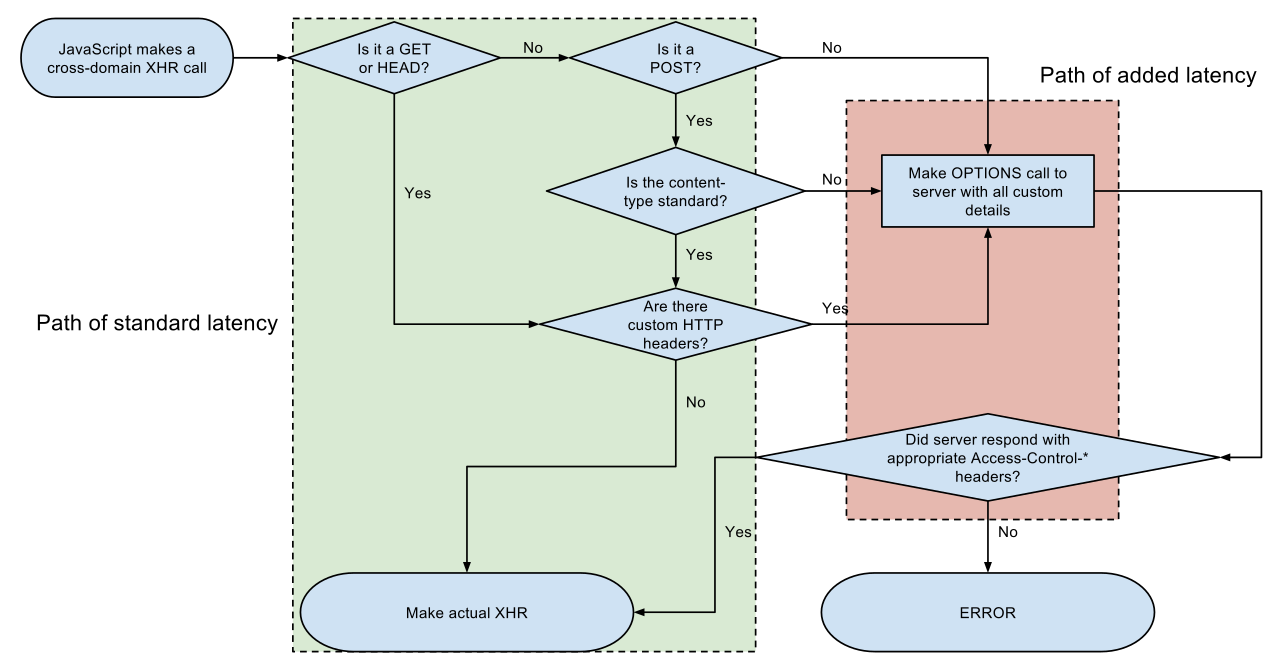
\includegraphics[width=\linewidth]{img/02_theorie/1280px-Flowchart_showing_Simple_and_Preflight_XHR.svg.png}
	\caption{Flowchart über den Ablauf von Ajax-Anfragen mit CORS \cite{FlowchartCORS}}
	\label{fig:cors-workflow}
\end{figure}

\subsubsection{Content-Security-Policy}

\nomenclature[Fachbegriff]{CSP}{Content-Security-Policy}
\nomenclature[Fachbegriff]{XSS}{Cross-Site-Scripting}
\nomenclature[Fachbegriff]{CDN}{Content Delivery Network}

Neben CORS gibt es im Browser eine Möglichkeit zu bestimmen, welche Funktionalitäten einer Webanwendung zur Verfügung stehen und wie diese vom Browser einzuschränken sind. Diese Funktion heißt Content-Security-Policy (CSP) und dient unter anderem dem Schutz vor Cross-Site-Scripting, indem eine Webanwendung beschränken kann, welche Funktionalitäten in JavaScript verfügbar sind und von wo aus Skripte und Daten geladen werden dürfen \cite{MDNContentSecurityPolicy}. Weiterhin kann bei einem Versuch diese Regeln zu umgehen, eine Berichterstattung darüber eingerichtet werden.

\subsection{Logdaten}
\label{sec:logdaten}

Ähnlich wie bei anderen Umgebungen gibt es eine standardisierte Log- bzw. Konsolenausgabe für die JavaScript-Umgebung \cite{MDNConsole}. Diese Ausgabe ist aber für den Standard-Benutzer unbekannt und es kann nicht erwartet werden, dass Nutzer dieses Log bereitstellen. Hinzukommend ist es, durch die zuvor beschrieben Härtungsmaßnahmen von Browsern, nicht möglich das Log direkt in eine Datei zu schreiben.

Um die Logdaten also zu erheben, gilt es entweder ein spezielles Log-Framework in der Webanwendung zu verwenden oder die bestehende Schnittstelle zu überschreiben oder zu wrappen. Nachdem die Datenerhebung gewährleistet ist, gilt es jedoch zudem die Daten an ein Partnersystem weiterzuleiten, welches die Beachtung der zuvor beschriebenen Einschränkungen erfordert. Alles in Allem stellt sich die Logdatenerhebung als nicht trivial dar, eine genauere Betrachtung erfolgt in der Untersuchung bestehender Lösungen.

\subsection{Fernzugriff}

Ein weiterer Punkt, der den \enquote{Browser} von anderen Umgebungen unterscheidet, ist, dass die Betreiber und Entwickler sich normalerweise nicht auf die Systeme der Nutzer schalten können. Bei Expertenanwendungen, bei denen die Nutzerschaft bekannt ist, ließe sich solch eine Funktionalität ggf. realisieren. Es gibt jedoch keine standardmäßige Funktionalität auf das gesetzt werden kann, wie z. B. das Remote Application Debugging \cite{JavaDebugWireProtocol} von Java. Weiterhin sind bei einer Webanwendung, die für den offenen Markt geschaffen ist, hierbei sind die Nutzer zahlreich sowie unbekannt und so eine Funktionalität lässt sich nicht realistisch umsetzen.